%
\begin{table}
	\caption{Difficulties of datasets: articulation, intra-class variance, background clutter and viewpoint variation}
	\label{tab:challenges}
	\begin{tabular}{l|rrrr}
		Dataset &  Articul.& Var. &  Backgr.& Viewp.  \\ \hline
		CelebA &   &  &  &    \\
		Cat Head & &  \checkmark&  &   \\
		CUB-200-2011 & & \checkmark& \checkmark&   \\
		Human3.6M &\checkmark& &  & \checkmark  \\
		BBC Pose &  \checkmark&  & \checkmark&  \\
		Dogs Run & \checkmark& \checkmark& \checkmark&   \\
		Penn Action & \checkmark& \checkmark& \checkmark& \checkmark\\
	\end{tabular}
\end{table}
%
% SHOW DISENTANGLING: SHAPE
\begin{figure}[t]
	\begin{subfigure}{0.5\textwidth}
	\centering
	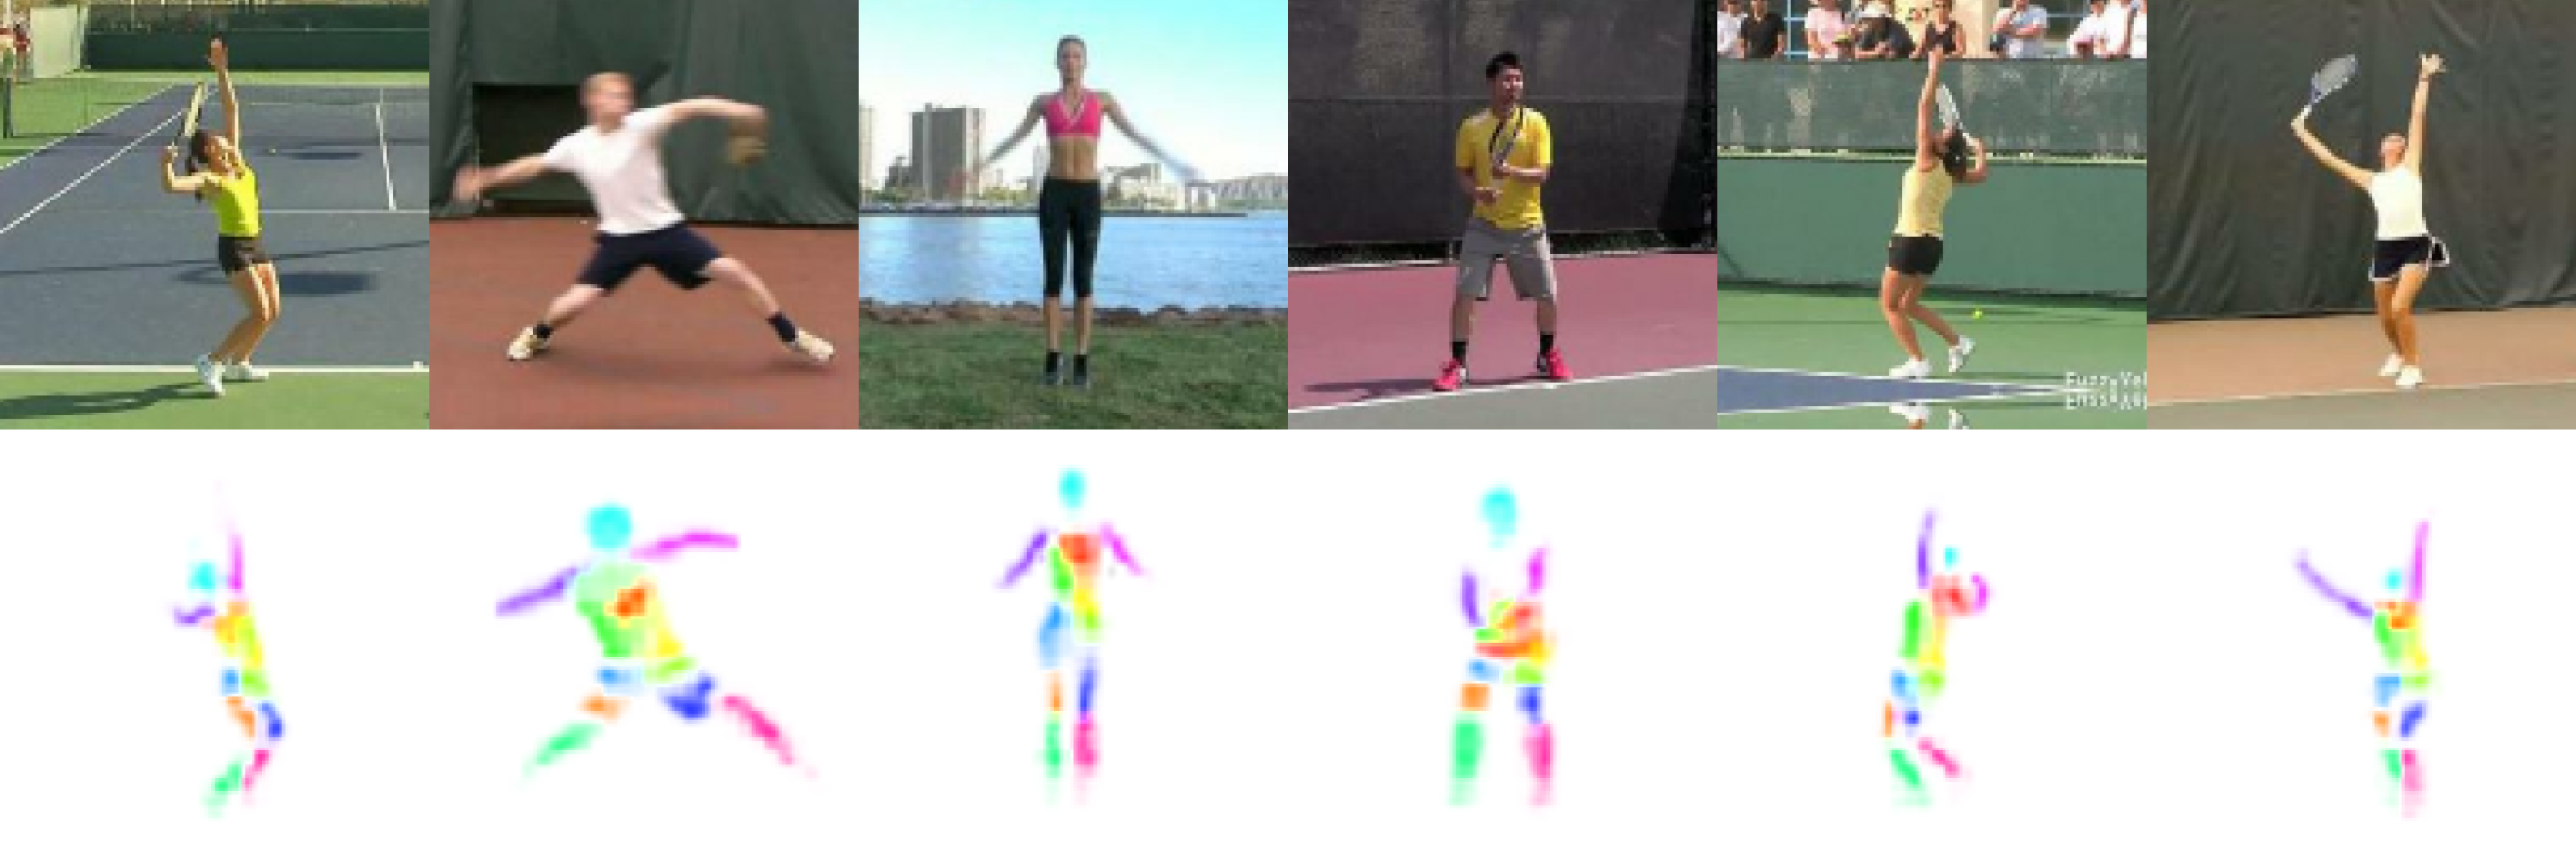
\includegraphics[trim={0cm 0cm 0cm 0cm},clip, width=1.\linewidth]{fig/shape6white}\caption{}
	\label{fig:shape_penn}
	\end{subfigure}
	\begin{subfigure}{0.5\textwidth}
	\centering
	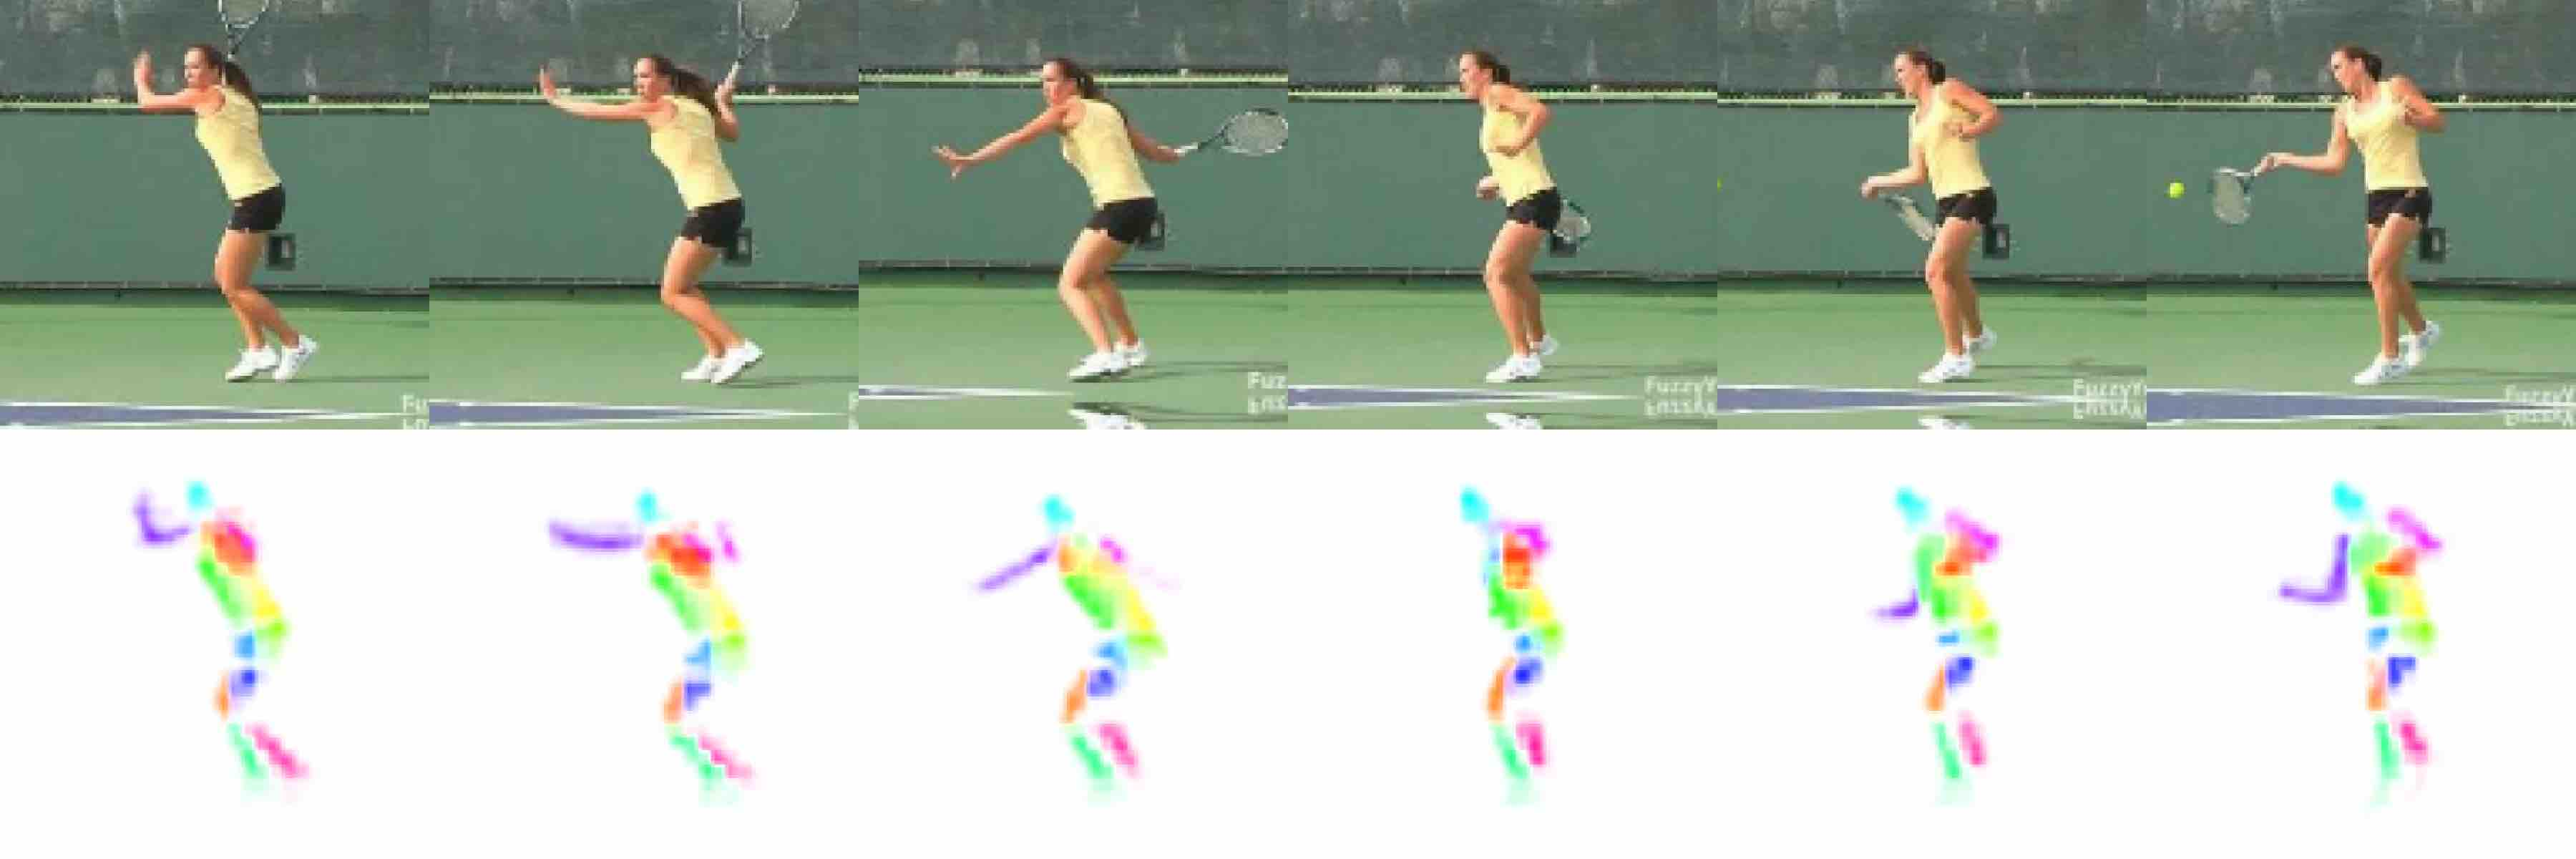
\includegraphics[trim={0cm 0cm 0cm 0cm},clip, width=1.\linewidth]{fig/shape_tennis}\caption{}
	\label{fig:shape_tennis}
	\end{subfigure}
	%\begin{subfigure}{0.5\textwidth}
	%\centering
	%\includegraphics[trim={0cm 0cm 0cm 0cm},clip, width=1.\linewidth]{mat/shape_yoga}\caption{}
	%\label{fig:shape_yoga}
	%\end{subfigure}
	\caption{Learned shape representation on Penn Action. For visualization, 13 of 16 part activation maps are plotted in one image. (a) Different instances, showing intra-class consistency and (b) video sequence, showing consistency and smoothness under motion, although each frame is processed individually.}
	\label{fig:shape}
\end{figure}
